%-----------------------------------------------------
% Chapter: Requirements Analysis
%-----------------------------------------------------
\chapter{Requirements Analysis}
\label{chap:requirements_analysis}
As the project involves the development of a prototype software solution, it is important to consider the project from a software engineering perspective. Moreover, the project involves the integration of a novel machine learning model, with the success of the project relying heavily on factors such as data availability, data quality and processing power. With this and other considerations such as training time and implementation complexity in mind, it is necessary to define software requirements to limit the project scope to one that is achievable. Software requirements should also be inferred from the needs of the end-user and as such it is necessary to understand user needs through existing solutions. This chapter briefly evaluates two existing solutions and outlines the functional and non-functional requirements by which the prototype will be evaluated.
\section{Existing Solutions}
\subsection{MasterWriter}
\begin{figure}[h]
	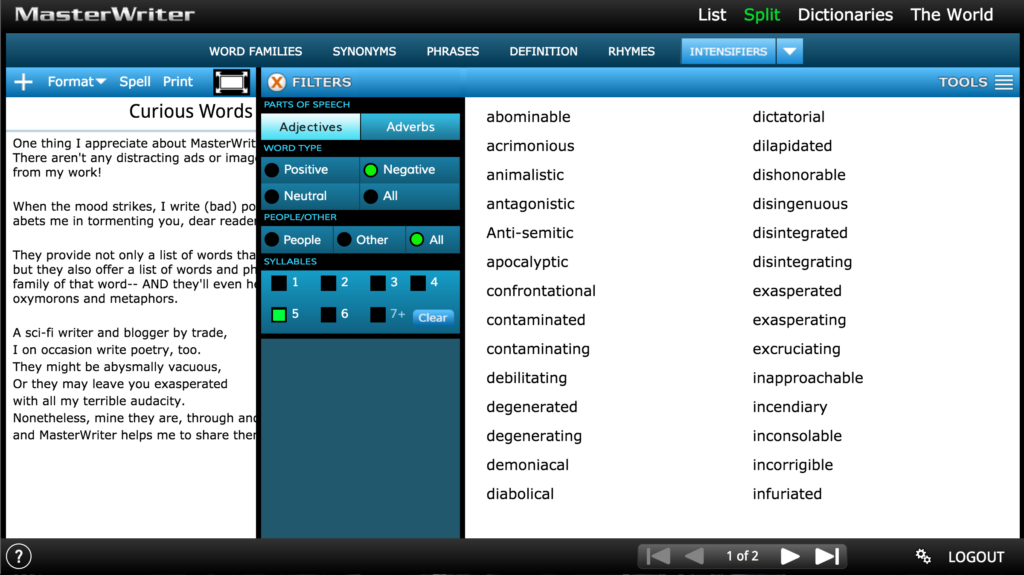
\includegraphics[width=10cm, height=6cm]{./figures/fig9}
	\centering
	\caption[MasterWriter]{MasterWriter user interface}
	\label{fig:fig9}
\end{figure}
\noindent
Self-described as \textbf{\textit{"The most powerful suite of writing tools ever assembled in one program."}}, MasterWriter is a software application aimed towards songwriters, poets and creative
writers. Available as a multi-platform product, it consolidates a number of writing aids into one application. Some of the core features of MasterWriter are highlighted in \autoref{Tab:MasterWriter} below.

\begin{table}[ht]
	\centering
	\begin{tabular}{ | l | p{10cm} |}
		\hline
		\textbf{Feature} & \textbf{Description}\\ \hline
		Word Dictionary & Provides a word dictionary with word
		definitions \\ \hline
		Rhyming Dictionary & Provides a rhyming dictionary with
		word/phrase rhymes \\ \hline
		Phrase Dictionary & Provides a phrase dictionary of predefined
		phrases \\ \hline
		Word Families & An extension of a typical thesaurus which
		provides a reference dictionary which can
		filter on subtle differences in word
		meanings \\ \hline
		Speech Types & Provides a predefined list of different
		figures of speech \\ \hline
		Synonyms & Provides a thesaurus containing
		synonyms\\ \hline
	\end{tabular}
	\label{Tab:MasterWriter}
	\caption{MasterWriter Features}
\end{table}

\noindent
\newline
\subsection{Rhymer's Block}

\begin{figure}[h]
	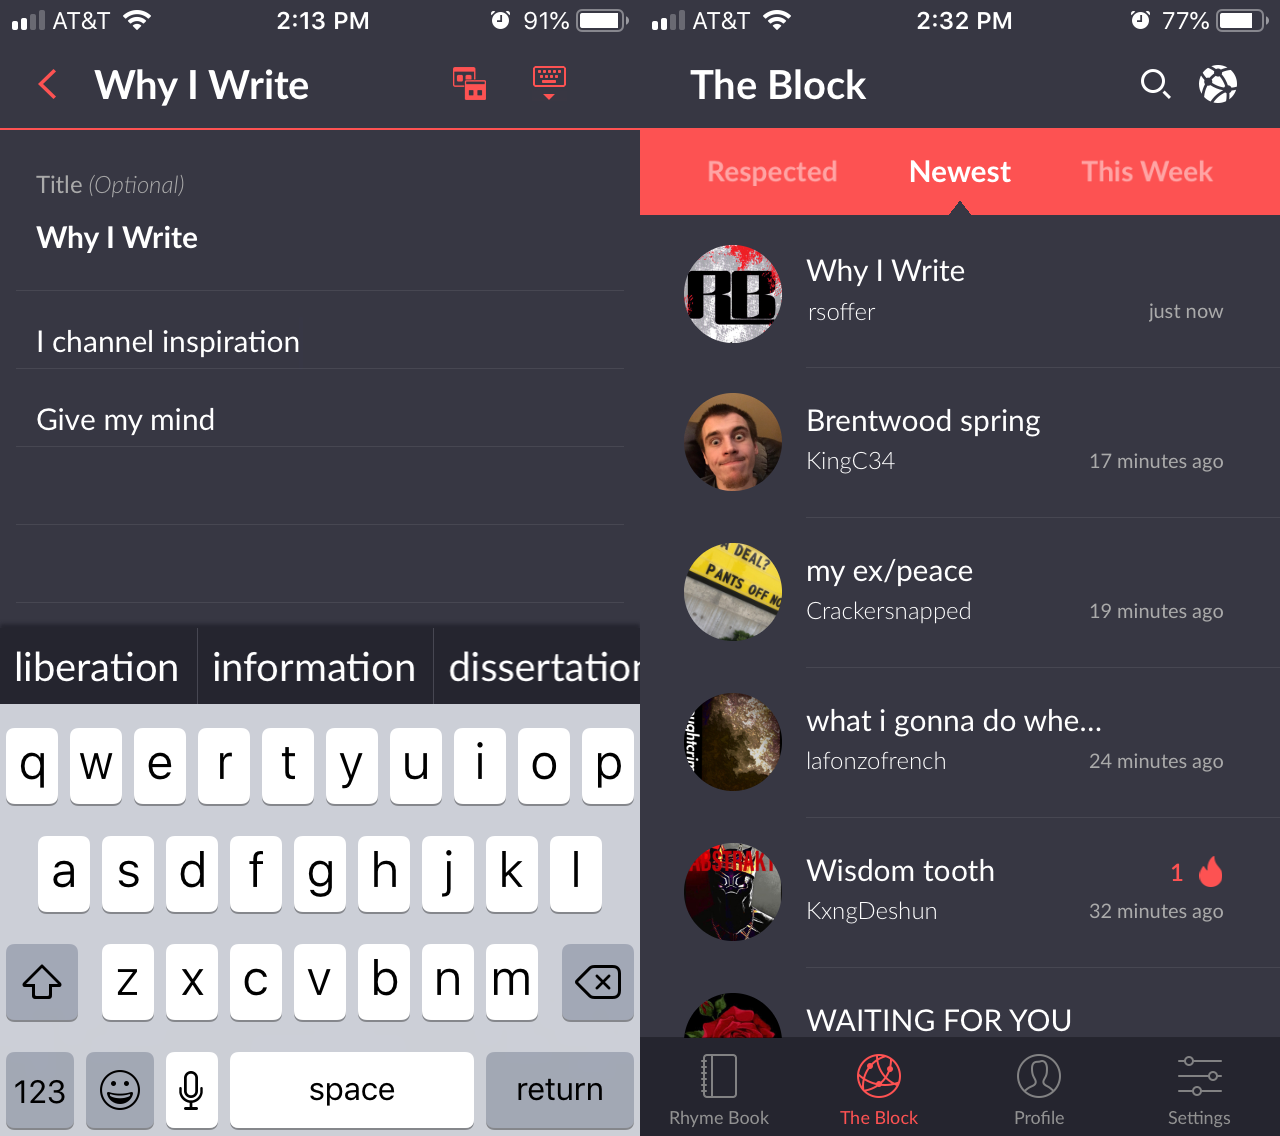
\includegraphics[width=10cm, height=9cm]{./figures/fig10}
	\centering
	\caption{Rhymer's Block}
	\label{fig:fig10}
\end{figure}
\noindent
\newline
Rhymer's block is a mobile application intended to help songwriters specifically with rhymes. Providing real time rhyme suggestions, the application allows users to quickly write song lyrics and provides a social platform through which users can share their own song lyrics, as well as review the song lyrics of other users. An overview of Rhymer's Block core features can be seen in \autoref{Tab:RhymersBlock}.

\begin{table}[ht]
	\centering
	\begin{tabular}{ | l | p{10cm} |}
		\hline
		\textbf{Feature} & \textbf{Description}\\ \hline
		Real-Time Rhyme Suggestion & Provides real time suggestions of rhyming words \\ \hline
		Cloud Storage & Provides cloud storage for a user's song lyrics \\ \hline
		Social Platform & Provides a online platform for users to share and comment on song lyrics\\ \hline
		Word Dictionary & Provides a word dictionary with word definitions \\ \hline
		Thesaurus & Provides a thesaurus containing synonyms\\ \hline
		Word Analysis & Provides rhyme suggestions for words most commonly used by other users \\ \hline
	\end{tabular}
	\label{Tab:RhymersBlock}
	\caption{Rhymer's Block Features}
\end{table}

\subsection{Requirements analysis}
Both MasterWriter and Rhymer's Block provide functionality for users to write, edit and save their lyrics. Similarly, both applications offer word search functionality to help writers with word choice, a primary issue highlighted before, through features such as rhyme suggestions, word dictionaries and thesauruses. Taking inspiration from both applications and as a basis for SONGIFAI, a lyric editor and word suggestion feature are mandatory for implementation. As previously stated, software applications like MasterWriter are static in nature, and fail to capture the dynamic nature of language. Examining Rhymer's Block, a particular feature deviates away from this, namely its real-time rhyme suggestions which leverages word usage within the application's online community. The implementation of a social platform is not in the scope of this project, however Rhmyer's Block usage of its users language is comparable to a goal of this project which is to help songwriters with their own lyrics, leveraging genre specific word embeddings.

\noindent
\newline
Neither MasterWriter or Rhymer's block address the secondary issue raised in \autoref{chap:intro}; namely helping songwriters with classifying their lyrics to help infer instrumental style. Whilst this project only considers three music genres, the potential application of such a feature becomes more apparent when considering sub-genres within music, which as explained in \autoref{chap:intro} is ever increasing. Though sub genres are out of scope for this project, a basic genre classification feature will be implemented for SONGIFAI which will classify a user's submitted song lyric as either Pop, Rock or Hip Hop.

\noindent
\newline
Comparing MasterWriter and Rhymer's block, software availability and accessibility are dealt with differently. Whilst MasterWriter offers its application on various platforms, Rhymer's Block utilises cloud storage for better accessibility. To address both software availability and accessibility, whilst keeping the project in scope, SONGIFAI will take the form of web application.  

\noindent
\newline
As a whole, the project has roots in both research and practice. Often times the interests of both these areas are incompatible. For example, research tends to focus more on advancing the current state of the art without paying too much attention to aspects such as model scalability, overall training time, ease of implementation and quality. On the other hand in practice applications  are for the most part client driven meaning aspects such as delivery time become important, and the performance of a model can be suboptimal if it is robust to train and easy to deploy to production. With regards to the project, necessary compromises, from both a research and application stand point have been made in order to achieve the goals of the project. For example a typical software solution would involve an iterative design process from a low fidelity prototype to a high fidelity prototype. As stated before the goals of this project are not client driven and due to further time constraints an iterative design process will not be adhered to. In the same vein, from a research perspective, techniques such as hyperparameter tuning through methods such as grid search will also not be followed; again due to time constraints and the type of models, (RNN's) that take time to train.

\noindent 
\newline
Taking into consideration the project goals and what has been discussed above, the project requirements are outlined below.
\section{Requirements}
In this section the requirements for the project are set out. The functional requirements specify what the software will do whilst the non-functional requirements will detail how these will be done. Possible extensions for the project, if time permits are also outlined.
\subsection{Functional}
\begin{table}[h]
	\centering
	\begin{tabular}{ | l | p{10cm} | l | }
		\hline
		\textbf{ID} & \textbf{Description} & \textbf{Dependency} \\ \hline
		FR1 & The system should allow users to input lyrics & N/A \\ \hline
		FR2 & The system should allow users to edit, save and delete lyrics & N/A  \\ \hline
		FR3 & The system should be able to classify user submitted lyrics as either Pop/Rock/Hip Hop & N/A \\ \hline
		FR4 & The system should be be able to suggest words from a given word. These words should be the most similar words in the chosen covariate word embedding space & N/A \\ \hline
		FR5 & The system should be able to provide real time text prediction whilst a user is in edit mode & N/A \\ \hline
		FR6 & The system should allow for the filtering of explicit content in both the word suggestion and word prediction feature & N/A \\ \hline
		FR7 & The user should be able to change the underlying covariate specific word embeddings used or the base embeddings if desired& N/A \\ \hline
	\end{tabular}
	\label{Tab:Tcru}
	\caption[Functional Requirements]{SONGIFAI Functional Requirements}
\end{table}
\subsection{Non-Functional}
\begin{table}[ht]
\centering
	\begin{tabular}{ | l | p{10cm} | l | }
		\hline
		\textbf{ID} & \textbf{Description} & \textbf{Dependency} \\ \hline
		NFR1 & The system should take the form of a web application, compatible on multiple device types & N/A \\ \hline
		NFR2 & The word prediction feature should return a list of candidate words with minimal latency & N/A \\ \hline
		NFR3 & The word suggestion feature should return a list of suggested words with minimal latency & N/A \\ \hline
	\end{tabular}
	\label{Tab:Tcr}
	\caption[Non-Functional Requirements]{SONGIFAI Non-Functional Requirements}
\end{table}
\subsection{Extensions}
\begin{table}[ht]
	\centering
	\begin{tabular}{ | l | p{10cm} | l | }
		\hline
		\textbf{ID} & \textbf{Description} & \textbf{Dependency} \\ \hline
		E1 & The system may allow rhyme words to be suggested in the word suggestion feature if time permits& N/A \\ \hline
		E2 & The system may allow sub genres to be selected for embeddings, if time and data permits& N/A \\ \hline
	\end{tabular}
	\label{Tab:Tcr}
	\caption[Possible Extensions]{SONGIFAI Possible Extensions}
\end{table}


